\section{Лабораторна робота 1. Типи даних. Інкапсуляція. Агрегація}
 

Аудиторний час на виконання лабораторної роботи --- 16 годин.

Мета роботи полягає у набутті практичних знань та навичок. 
До знань належать:
\begin{enumerate}
\item розуміння змінних, примітивних (цілих, дійсних, булевих), непримітивних (об’єктів, масивів, перелічуваних) типів даних та операторів над ними;
\item правила допустимого іменування змінних;
\item область видимості змінних;
\item зарезервовані імена (ключові слова). 
\end{enumerate}

До практичних навичок належать:
\begin{enumerate}
\item Створення виконуваних класів, їхньої компіляції та виконання в середовищі JDK.
\item Створення класів, що інкапсулюють поля різних типів.
\item Реалізація принципу агрегації засобами масивів.
\end{enumerate}

\subsection{Постановка задачі}
Слід розробити консольний (J2SE) додаток, в якому обов’язково повинно бути не менше двох класів, оголошених в різних файлах. Один з цих класів повинен бути виконуваним, а інший --- класом-моделлю (структурою даних).

Виконуваний клас повинен створити масив об’єктів модельного класу, встановлюючи їхні поля у випадкові значення, а потім висвітлити їх на екрані.

\subsection{Теоретичні відомості}
Основою будь-якої прикладної програми у Java є виконуваний клас. Виконуваним вважається клас, який є загальнодоступним (public), тобто видимим за межами власного пакету (докладніше про пакети і видимість --- згодом), а також містить статичну функцію
\begin{lstlisting}
public static void main(String[]a){/* code */}
\end{lstlisting}
або
\begin{lstlisting}
public static void main(String a[]){/* code */}
\end{lstlisting}
або
\begin{lstlisting}
public static void main(String ...a){/* code */}
\end{lstlisting}

У лістингу 1 наведено приклад простого виконуваного класу.

{\bf Лістинг 1.
Приклад виконуваного класу }
\begin{lstlisting}
public class Welcome{
    public static void main(String...a){
        System.out.println("Welcome, dear "+
            "third-form students of PZAS!");
    }
}
\end{lstlisting}
Первинний код класу можна підготувати у будь-якому текстовому редакторі, навіть у notepad, хоча суттєво зручніше працювати у редакторі, що виділяє мовні конструкції кольором, наприклад, Notepad++ або у інтегрованому середовищі розробки, наприклад, Eclipse чи IntelliJ IDEA. Проте, майте на увазі, що це повинен бути справді текстовий редактор (англійською plain text editor), а не текстові процесори на зразок MS Word, які добавляють до текстів спеціальні символи форматування.
Імена файла та виконуваного класу, що в ньому знаходиться повинні співпадати. Файл мусить мати розширення ``.java''. Наприклад, первинний код виконуваного класу з лістингу 1 повинен бути збереженим будь-де у файлі з назвою Welcome.java. 
Компіляція первинного коду у байт-код, придатний до виконання віртуальною машиною Java (JVM) можна здійснити у середовищі розробки або з командного рядка.

Якщо Ви вирішили працювати у середовищі Ecilpse чи IDEA, то запустіть його. Ми рекомендуємо користуватися IntelliJ IDEA Community Edition для розробки під JavaSE та Android Studio для розробки під Android, оскільки вони мають хороші засоби інспекції коду, рефакторингу, використовують сучасну технологію збирання gradle з репозиторіями модулів повторного використання maven. 

Створіть новий проект, клацнувши на кнопку Create New Project.
Вкажіть ``App by <Ваше прізвище>'' як назву проекту. Звісно вставте Ваше справжнє прізвище замість <Ваше прізвище>. 
У полі Project location вкажіть шлях до каталогу, де будуть зберігатися файли проекту. Будь ласка, встановіть цей шлях на носії, що придатний для довготривалого збереження даних, бо ці файли будуть використовуватися для оцінювання Вашої роботи.
У випадаючому списку Project SDK оберіть 1.7 (java version "1.7.x\_xx") або 1.8 (java version "1.8.x\_xx"). Клацніть next, finish і в ``Project explorer'' Ви побачите, що новий проект створено.
 
Розширте список його файлів, клацнувши трикутничок ліворуч від назви проекту \img{exposeProject}. 
 Потім клацніть правою клавішею на ``src'', оберіть New->Package і створіть пакет ``com.<Ваше прізвище>.myapp''. В схожий спосіб, клацнувши правою клавішею на пакеті, який щойно утворився, створіть підпакети ``model'', ``util'' та ``application''.
 
За допомогою контекстного меню New->Java Class створіть клас App в пакеті application. Після натиснення ``OK'', появиться вікно редагування коду класу. Модифікуйте його відповідно до лістингу 1.
Клацніть на кнопку ``Make'', що схематично показана зеленою стрілочкою вниз та двійковими числами. Після закінчення процесу збирання, оберіть праворуч із випадаючого списку  конфігурацію ``App'' і клацніть зелену кнопку-трикутничок ``Run''.
 
Після запуску програми побачите результат її виконання у віконці Console.

Якщо у Вас, з якихось причин, немає доступу до інтегрованого середовища розробки, наберіть лістинг 1 у будь-якому текстовому редакторі, збережіть його у папці com/<Ваше прізвище>/lab1/application і виконайте компіляцію з командного рядка: 

javac App.java

Примітка: якщо Ви працюєте в ОС, що ігнорує регістр букв у назвах файлів, то компіляцію можна виконати й командою javac app.java або, навіть JaVaC aPp.jAvA

Якщо результатом спроби компіляції є повідомлення про те, що javac не є ні внутрішньою, ні зовнішньою командою, ні виконуваною програмою, ні пакетним файлом, то або Ви не встановили JDK або не налаштовано змінну середовища з шляхом до його виконуваних файлів. Дізнатись про те, де отримати JDK і як налаштувати змінну середовища PATH можна з додатку~А.

Після виконання компіляції у поточній директорії появиться файл App.class, що містить байт-код виконуваного класу. Щоб запустити клас на виконання слід у командному рядку написати 

java -cp <шлях/до/папки/com> com.<Ваше прізвище>.myapp.application.App

або, коли <шлях/до/папки/com> записано в змінній середовища CLASSPATH, то просто

java com.<Ваше прізвище>.myapp.application.App

Примітка: на відміну від команди компілювання, команда запуску виконуваного класу чутлива до регістру букв у його назві. Це справедливо для всіх платформ, навіть MS Windows.

\subsection{Види модельних класів}
\begin{enumerate}
\item особа (ім’я, стать, рік народження);
\item працівник з полями:
	\begin{itemize}
	\item прізвище (String),
	\item ім’я (String),
	\item рік прийому на роботу (Integer),
	\item рік народження (Integer),
	\item основне місце роботи (String)
	\end{itemize}
\item овоч (сорт, вага, колір, умовне позначення у вигляді unicode-стрічки);
\item транспортний засіб (вид, бренд, вага, колір, умовне позначення у вигляді unicode-стрічки, рік виготовлення);
\item ґаджет (вид, бренд, вага, розміри і принцип дії сенсорного екрану, об’єм оперативної пам’яті, частота і кількість ядер ЦП, вид і потужність акумуляторної батареї).
\end{enumerate}

\subsection{Хід роботи}
Напишіть програму на мові Java в якій будуть наступні модулі (файли *.java з текстом класів):
\begin{enumerate}
\item модельний клас, наприклад, Працівник, в пакеті com.<Ваше прізвище>.myapp.model

В класі повинен бути переозначений метод toString() в такий спосіб, щоб він повертав інформацію про працівника у вигляді читабельної стрічки; всі поля повинні бути інкапсульовані і доступні за допомогою методів getters-setters;
\item  клас com.<Ваше прізвище>.myapp.util.WorkerBuilder, що реалізує зразок проектування (дизайн паттерн) builder в такий спосіб, що можна створювати працівників за допомогою конструкції на зразок:
\begin{lstlisting}
Worker worker = new WorkerBuilder().surname("Pigovsky")
    .names("Yuriy Romanovych")
        .yearOfBirth(1983)
            .yearOfEmployment(2004)
                .build();
\end{lstlisting}
\item статичний метод WorkerBuilder.generateWorkers(), що, користуючись вищезгаданим WorkerBuilder, повертає масив 10 працівників з випадковими іменами і датами народження 
\item виконуваний клас com.<Ваше прізвище>.myapp.application.App, що у своїй функції main виводить в консоль всіх працівників, згенерованих методом WorkerBuilder.generateWorkers()
\end{enumerate}

 При реалізації методів доступу (getters, setters) до  полів класу Worker користуйтеся  рефакторінгом. Натисніть комбінацію клавіш <Alt>+<Insert> та виберіть ``Generate getters and setters''.
Відзначне галочками потрібні поля, клацніть ОК і до тексту класу добавляться методи доступу на зразок
\begin{lstlisting}
    public void setSurname(String surname) {
        this.surname = surname;
    }
    public String getSurname() {
        return surname;
    }
\end{lstlisting}

Для того, щоб створити конструктор, що ініціалізує будь-які чи всі поля класу натисніть, знаходячись у файлі з класом, комбінацію клавіш <Alt>+<Insert> (або оберіть з контекстного меню опцію Generate) і клацніть ``Constructor''. У вікні, що появиться, виділіть необхідні поля і натисніть Refactor.

Щоб створити WorkerBuilder оберіть з контекстного меню Refactor->Replace constructor with builder...


Для автоматичного форматування тексту програми  натисніть комбінацію клавіш <Ctrl>+<L>. 

Вивід в консоль виконуйте методом System.out.println().

Переозначення методу toString можна виконати написавши частину його імені, наприклад, ``to'', в тексті класу і натиснувши комбінацію кнопок автодоповнення <Ctrl>+<ПРОБІЛ>. Цим же способом можна користовуватися для автодоповнення імен, визначення списку аргументів метода і т.д. Комбінація кнопок <Ctrl>+<Q> показує швидку підказку до метода на якому стоїть курсор, а <Ctrl>+<P> показує набір його аргументів.

\subsection{Порядок виконання програми}
Програма повинна запускатися з класу ``App'', тобто він виступає виконуваним класом. Після запуску програми функція main повинна у циклі друкувати всіх працівників, що були згенеровані методом WorkerBuilder.generateWorkers(). 

\subsection{Додаткові завдання з конструювання ПЗ}
\begin{enumerate}
\item Всі файли з сирцевими кодами повинні бути оформлені відповідно до конвенції [\url{http://www.oracle.com/technetwork/java/codeconvtoc-136057.html}]
\item Перед кожним класом, полем і методом повинні бути javadoc [\url{http://www.oracle.com/technetwork/java/javase/documentation/index-137868.html}] коментарі з читабельним і зрозумілим описом, наприклад:
\begin{lstlisting}
/**
 * Constructs a person with all his (her) properties
 * @param surname if unknown --- can be null
 * @param names a parson can have several names separated 
 * with a space
 * @param yearOfBirth if unknown --- can be null
 * @param yearOfEmployment year, when the person was
 * appointed to a post
 * @param mainWorkplace the name of a company, where 
 * the person works
 */
public Worker(String surname, String names, 
        Integer yearOfBirth, Integer yearOfEmployment, 
            String mainWorkplace) {
    this.surname = surname;
    this.names = names;
    this.yearOfBirth = yearOfBirth;
    this.yearOfEmployment = yearOfEmployment;
    this.mainWorkplace = mainWorkplace;
}
\end{lstlisting}
Тоді сторінка документації, що появляється при натиску комбінації клавіш <Ctrl>+<Q> на ідентифікаторі у вікні редактора, буде вигладати так:
\begin{figure}[H]
\centering
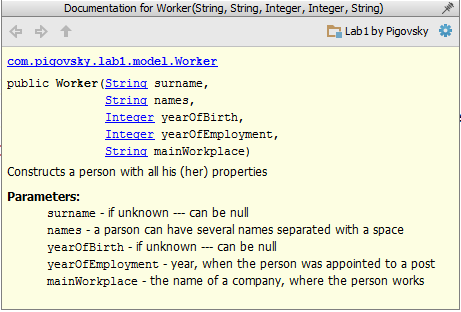
\includegraphics{JavadocExample}
\end{figure}

\item Потрібно створити JUnit тест-кейс, що перевіряє вірність роботи WorkerBuilder, тобто чи він дає вірні значення за замовчуванням для незаданих полів.
\end{enumerate}

JUnit тест можна створити натиснувши комбінацію клавіш <Ctrl>+<Shift>+<T>, перебуваючи у файлі з класом, до якого плануєте написати тест. Після цього, у контекстному меню, що появилося, слід натиснути ``Create new test''. 

У вікні створення теста оберіть JUnit4 навпроти Testing library. Ім'я класу залиште WorkerBuilderTest, назвою цільового пакету вкажіть com.<Ваше прізвище>.myapp.test. Поставте галочки навпроти setUp/@Before та у списку ``Generate test methods for:'' відзначте build(): Worker, як показано на рисунку
\begin{figure}[H]
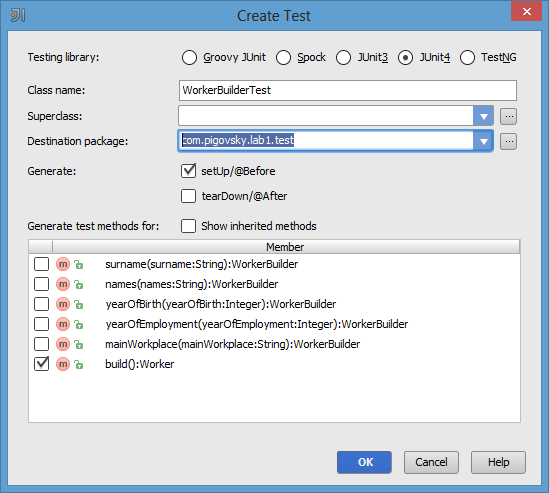
\includegraphics{createTest}
\end{figure}
Появиться вікно з текстом тесткейсового класу. Перш за все, після оголошення пакету, добавте оператор статичного імпортування функцій перевірки:
\begin{lstlisting}
import static org.junit.Assert.*;
\end{lstlisting}
Це дозволить звертатися до функцій на зразок Assert.assertEquals(...) за коротшим іменем assertEquals(...).

Метод setUp() буде викликатися перед запуском кожного тестового методу. Запишіть у ньому створення екземпляру об'єкта WorkerBuilder.

У методі testBuild задайте об'єкту-білдеру лише прізвище працівника (без року народження чи року прийняття на роботу) і побудуйте об'єкт працівника. Перевірте методом assertNull чи роки народження і прийняття на роботу мають очікуване неозначене null.
В результаті цих дій у Вас має утворитися щось на зразок нижчеподаного лістингу

\begin{lstlisting}
package com.pigovsky.lab1.test;

import com.pigovsky.lab1.model.Worker;
import com.pigovsky.lab1.model.WorkerBuilder;
import org.junit.Before;
import org.junit.Test;

import static org.junit.Assert.*;

/**
 * Tests if builder provides expected defaults
 */
public class WorkerBuilderTest {
    private WorkerBuilder builder;

    @Before
    public void setUp() throws Exception {
        builder = new WorkerBuilder();
    }

    @Test
    public void testBuild() throws Exception {
        Worker worker = builder.surname("Pigovsky").
                build();
        assertNull("Year of birth is not null, but " +
                "it should be null by default!",
                worker.getYearOfBirth());
        assertNull("Year of appointment is " +
                "not null, but it should be " +
                "null by default!",
                worker.getYearOfEmployment());
    }
}
\end{lstlisting}

Спробуйте запустити тест. Для цього Вам доведеться створити нову конфігурацію запуску і задати Test kind в положення ``All in package'', як показано на рисунку
\begin{figure}[H]
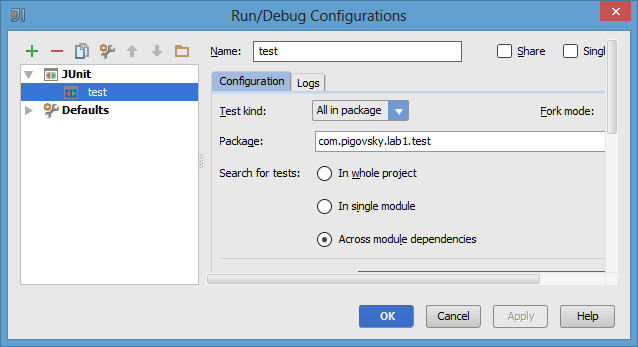
\includegraphics{testRunConfiguration}
\end{figure}

Тестування повинно пройти успішно, про що свідчитиме зелений progress bar. Після цього замініть значення років по-замовчуванню в класі WorkerBuilder на будь-що відмінне від неозначеного null, наприклад, на 0 (число нуль).
При повторному тестуванні, Ви мали би отримати повідомлення, схоже на ``java.lang.AssertionError: Year of appointment is not null, but it should be null by default!''.


В класі Worker cтворіть метод getAge(), який рахує вік працівника за роком народження. При цьому, треба бути завбачливим і врахувати, що Вашою програмою можуть користуватися більше як один рік. Тому для отримання поточного року використайте виклик на зразок
\begin{lstlisting}
int currentYear = Calendar.getInstance().get(Calendar.YEAR);
\end{lstlisting}

Для тестування методу getAge, створіть ще один тест-кейс, як Ви це вже робили для методу build. Приклад тест-кейсу наведено у лістингу:
\begin{lstlisting}
package com.pigovsky.lab1.test;

import com.pigovsky.lab1.model.WorkerBuilder;
import org.junit.Test;

import static org.junit.Assert.assertEquals;

/**
 * Tests if age is computed correctly
 */
public class WorkerTest {
    @Test
    public void testGetAge() throws Exception {
        assertEquals(32, new WorkerBuilder().
                yearOfBirth(1983).
                    build().
                        getAge());
    }
}
\end{lstlisting}

\subsection{Зміст звіту}

Звітом з виконання лабораторної роботи є файли проекту в оприлюдниному репозиторії (див. розділ {\bf Загальні принципи звітування і оцінювання лабораторних робіт з ``Технології Java''}.
 
